% This is part of Un soupçon de mathématique sans être agressif pour autant
% Copyright (c) 2015
%   Laurent Claessens
% See the file fdl-1.3.txt for copying conditions.

\begin{mental}
    Répartition des animaux dans un zoo :
    \begin{center}
    \begin{tabular}[]{|c||c|}
        \hline
        proportion (en \%)&type\\
        \hline\hline
        \( 13\)&reptiles\\
        \hline
        \ldots&oiseaux\\
        \hline
        60&mammifères\\
        \hline
        9&poissons\\
        \hline
    \end{tabular}
    \end{center}


    \begin{enumerate}
        \item
            Compléter le tableau
        \item
            Laquelle des deux représentations est correcte ?

            \begin{center}
                
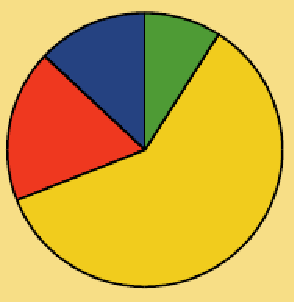
\includegraphics[width=6cm]{53_diag.pdf}
\hspace{2cm}
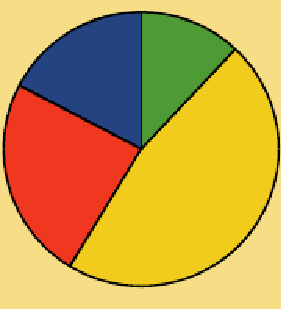
\includegraphics[width=6cm]{54_diag.pdf}
            \end{center}
            

    \end{enumerate}
    
\end{mental}
